% Options for packages loaded elsewhere
\PassOptionsToPackage{unicode}{hyperref}
\PassOptionsToPackage{hyphens}{url}
%
\documentclass[
]{article}
\usepackage{amsmath,amssymb}
\usepackage{lmodern}
\usepackage{ifxetex,ifluatex}
\ifnum 0\ifxetex 1\fi\ifluatex 1\fi=0 % if pdftex
  \usepackage[T1]{fontenc}
  \usepackage[utf8]{inputenc}
  \usepackage{textcomp} % provide euro and other symbols
\else % if luatex or xetex
  \usepackage{unicode-math}
  \defaultfontfeatures{Scale=MatchLowercase}
  \defaultfontfeatures[\rmfamily]{Ligatures=TeX,Scale=1}
  \setmainfont[]{NanumGothic}
\fi
% Use upquote if available, for straight quotes in verbatim environments
\IfFileExists{upquote.sty}{\usepackage{upquote}}{}
\IfFileExists{microtype.sty}{% use microtype if available
  \usepackage[]{microtype}
  \UseMicrotypeSet[protrusion]{basicmath} % disable protrusion for tt fonts
}{}
\makeatletter
\@ifundefined{KOMAClassName}{% if non-KOMA class
  \IfFileExists{parskip.sty}{%
    \usepackage{parskip}
  }{% else
    \setlength{\parindent}{0pt}
    \setlength{\parskip}{6pt plus 2pt minus 1pt}}
}{% if KOMA class
  \KOMAoptions{parskip=half}}
\makeatother
\usepackage{xcolor}
\IfFileExists{xurl.sty}{\usepackage{xurl}}{} % add URL line breaks if available
\IfFileExists{bookmark.sty}{\usepackage{bookmark}}{\usepackage{hyperref}}
\hypersetup{
  pdftitle={Field research},
  pdfauthor={이진주},
  hidelinks,
  pdfcreator={LaTeX via pandoc}}
\urlstyle{same} % disable monospaced font for URLs
\usepackage[margin=1in]{geometry}
\usepackage{color}
\usepackage{fancyvrb}
\newcommand{\VerbBar}{|}
\newcommand{\VERB}{\Verb[commandchars=\\\{\}]}
\DefineVerbatimEnvironment{Highlighting}{Verbatim}{commandchars=\\\{\}}
% Add ',fontsize=\small' for more characters per line
\usepackage{framed}
\definecolor{shadecolor}{RGB}{248,248,248}
\newenvironment{Shaded}{\begin{snugshade}}{\end{snugshade}}
\newcommand{\AlertTok}[1]{\textcolor[rgb]{0.94,0.16,0.16}{#1}}
\newcommand{\AnnotationTok}[1]{\textcolor[rgb]{0.56,0.35,0.01}{\textbf{\textit{#1}}}}
\newcommand{\AttributeTok}[1]{\textcolor[rgb]{0.77,0.63,0.00}{#1}}
\newcommand{\BaseNTok}[1]{\textcolor[rgb]{0.00,0.00,0.81}{#1}}
\newcommand{\BuiltInTok}[1]{#1}
\newcommand{\CharTok}[1]{\textcolor[rgb]{0.31,0.60,0.02}{#1}}
\newcommand{\CommentTok}[1]{\textcolor[rgb]{0.56,0.35,0.01}{\textit{#1}}}
\newcommand{\CommentVarTok}[1]{\textcolor[rgb]{0.56,0.35,0.01}{\textbf{\textit{#1}}}}
\newcommand{\ConstantTok}[1]{\textcolor[rgb]{0.00,0.00,0.00}{#1}}
\newcommand{\ControlFlowTok}[1]{\textcolor[rgb]{0.13,0.29,0.53}{\textbf{#1}}}
\newcommand{\DataTypeTok}[1]{\textcolor[rgb]{0.13,0.29,0.53}{#1}}
\newcommand{\DecValTok}[1]{\textcolor[rgb]{0.00,0.00,0.81}{#1}}
\newcommand{\DocumentationTok}[1]{\textcolor[rgb]{0.56,0.35,0.01}{\textbf{\textit{#1}}}}
\newcommand{\ErrorTok}[1]{\textcolor[rgb]{0.64,0.00,0.00}{\textbf{#1}}}
\newcommand{\ExtensionTok}[1]{#1}
\newcommand{\FloatTok}[1]{\textcolor[rgb]{0.00,0.00,0.81}{#1}}
\newcommand{\FunctionTok}[1]{\textcolor[rgb]{0.00,0.00,0.00}{#1}}
\newcommand{\ImportTok}[1]{#1}
\newcommand{\InformationTok}[1]{\textcolor[rgb]{0.56,0.35,0.01}{\textbf{\textit{#1}}}}
\newcommand{\KeywordTok}[1]{\textcolor[rgb]{0.13,0.29,0.53}{\textbf{#1}}}
\newcommand{\NormalTok}[1]{#1}
\newcommand{\OperatorTok}[1]{\textcolor[rgb]{0.81,0.36,0.00}{\textbf{#1}}}
\newcommand{\OtherTok}[1]{\textcolor[rgb]{0.56,0.35,0.01}{#1}}
\newcommand{\PreprocessorTok}[1]{\textcolor[rgb]{0.56,0.35,0.01}{\textit{#1}}}
\newcommand{\RegionMarkerTok}[1]{#1}
\newcommand{\SpecialCharTok}[1]{\textcolor[rgb]{0.00,0.00,0.00}{#1}}
\newcommand{\SpecialStringTok}[1]{\textcolor[rgb]{0.31,0.60,0.02}{#1}}
\newcommand{\StringTok}[1]{\textcolor[rgb]{0.31,0.60,0.02}{#1}}
\newcommand{\VariableTok}[1]{\textcolor[rgb]{0.00,0.00,0.00}{#1}}
\newcommand{\VerbatimStringTok}[1]{\textcolor[rgb]{0.31,0.60,0.02}{#1}}
\newcommand{\WarningTok}[1]{\textcolor[rgb]{0.56,0.35,0.01}{\textbf{\textit{#1}}}}
\usepackage{graphicx}
\makeatletter
\def\maxwidth{\ifdim\Gin@nat@width>\linewidth\linewidth\else\Gin@nat@width\fi}
\def\maxheight{\ifdim\Gin@nat@height>\textheight\textheight\else\Gin@nat@height\fi}
\makeatother
% Scale images if necessary, so that they will not overflow the page
% margins by default, and it is still possible to overwrite the defaults
% using explicit options in \includegraphics[width, height, ...]{}
\setkeys{Gin}{width=\maxwidth,height=\maxheight,keepaspectratio}
% Set default figure placement to htbp
\makeatletter
\def\fps@figure{htbp}
\makeatother
\setlength{\emergencystretch}{3em} % prevent overfull lines
\providecommand{\tightlist}{%
  \setlength{\itemsep}{0pt}\setlength{\parskip}{0pt}}
\setcounter{secnumdepth}{5}
\usepackage[hangul]{kotex}
\ifluatex
  \usepackage{selnolig}  % disable illegal ligatures
\fi

\title{Field research}
\usepackage{etoolbox}
\makeatletter
\providecommand{\subtitle}[1]{% add subtitle to \maketitle
  \apptocmd{\@title}{\par {\large #1 \par}}{}{}
}
\makeatother
\subtitle{This is subtitle}
\author{이진주}
\date{24 June, 2021}

\begin{document}
\maketitle

{
\setcounter{tocdepth}{2}
\tableofcontents
}
\hypertarget{uxc5f0uxad6c-uxac1cuxc694}{%
\section{연구 개요}\label{uxc5f0uxad6c-uxac1cuxc694}}

\begin{itemize}
\item
  R 프로그램을 이용하여 다양한 연구 결과를 종합, 정리하여 표준화할 수
  있음.
\item
  합성생물학 분야의 대회인 iGEM 사례를 분석하며 R 프로그램을 이용해
  데이터를 처리, 분석할 수 있음.
\item
  iGEM은 합성생물학 발전의 원동력이 되었다고 볼 수 있는데, 바이오파트를
  표준화하거나 이를 이용한 유전자회로를 설계, 환경이나 보건 등의 목표를
  가지고 연구하는 대회임.
\item
  이번 현장연구 수업에서는 iGEM 연구팀 중 특정 바이오파트를 이용한
  연구에 대한 데이터를 수집하고 이를 통합하여 데이터를 분석하고자 함.
\end{itemize}

\hypertarget{uxc5f0uxad6cuxc758-uxd544uxc694uxc131}{%
\subsection{연구의 필요성}\label{uxc5f0uxad6cuxc758-uxd544uxc694uxc131}}

\hypertarget{uxc0dduxbb3c-uxbd84uxc57cuxb294-uxc2dcuxc2a4uxd15cuxc758-uxbcf5uxc7a1uxc131-uxb54cuxbb38uxc5d0-uxc2e4uxd5d8-uxc7acuxd604uxc774-uxd798uxb4ec.-uxb530uxb77cuxc11c-uxc5ecuxb7ec-uxc5f0uxad6cuxc790uxb4e4uxc758-uxbc18uxbcf5-uxc2e4uxd5d8uxc744-uxd1b5uxd574-uxd2b9uxc815-uxbc14uxc774uxc624uxd30cuxd2b8uxc758-uxd45cuxc900uxd654uxac00-uxd544uxc694uxd568.}{%
\subsubsection{생물 분야는 시스템의 복잡성 때문에 실험 재현이 힘듬.
따라서 여러 연구자들의 반복 실험을 통해 특정 바이오파트의 표준화가
필요함.}\label{uxc0dduxbb3c-uxbd84uxc57cuxb294-uxc2dcuxc2a4uxd15cuxc758-uxbcf5uxc7a1uxc131-uxb54cuxbb38uxc5d0-uxc2e4uxd5d8-uxc7acuxd604uxc774-uxd798uxb4ec.-uxb530uxb77cuxc11c-uxc5ecuxb7ec-uxc5f0uxad6cuxc790uxb4e4uxc758-uxbc18uxbcf5-uxc2e4uxd5d8uxc744-uxd1b5uxd574-uxd2b9uxc815-uxbc14uxc774uxc624uxd30cuxd2b8uxc758-uxd45cuxc900uxd654uxac00-uxd544uxc694uxd568.}}

\hypertarget{synthetic-biology-is-invention}{%
\subsubsection{Synthetic Biology is
INVENTION!}\label{synthetic-biology-is-invention}}

-- 합성생물학은 생물학에 공학적 개념을 적용함으로써 생물 시스템을 비교적
예측 가능하도록 만들기 위한 분야임.

-- 전통적인 생물 실험이 연역적인 실험과 관찰, 발견에 기반했다면
합성생물학에서는 특정 목적을 위해 생물 시스템을 설계, 합성함으로써
발명의 측면으로 볼 수 있음

-- 발명의 측면에서 보자면 vector map은 설계도, 즉 blueprint에 비유할 수
있으며 logic gate는 설계한 시스템의 기능적 의미를 담고 있음.

\hypertarget{producibility-repeatability}{%
\subsubsection{Producibility \&
Repeatability}\label{producibility-repeatability}}

-- Producibility : 다른 사람이 동일한 실험을 했을 때 동일한 결과가 나옴.

-- Repeatability : 한 사람이 동일한 실험을 했을 때 동일한 결과가 반복됨.

\begin{itemize}
\tightlist
\item
  Rmarkdown의 철학과 필요성에 대한 참고영상
\end{itemize}

link :
\url{https://www.youtube.com/watch?v=s9aWmU0atlQ\&ab_channel=RStudio}

\begin{itemize}
\tightlist
\item
  Replication Crisis : 반복성 없는 실험 (irreproducible research)에 의한
  연구비 등의 소모
\end{itemize}

\hypertarget{uxc5f0uxad6c-uxbaa9uxd45c}{%
\subsection{연구 목표}\label{uxc5f0uxad6c-uxbaa9uxd45c}}

\begin{itemize}
\item
  해당 현장연구 수업을 통해 합성생물학의 개념을 정립하고, 사용된
  부품/회로들의 정량적 데이터를 수집하여 재현성을 분석할 수 있음.
\item
  데이터를 수집, 분석하는 과정에서 Rmarkdown/Rstudio를 활용한다.
\end{itemize}

\begin{center}\rule{0.5\linewidth}{0.5pt}\end{center}

\hypertarget{uxc5f0uxad6c-uxbc29uxbc95}{%
\section{연구 방법}\label{uxc5f0uxad6c-uxbc29uxbc95}}

\hypertarget{uxc5f0uxad6c-uxbc29uxbc95-1-data-collection_igem-rmarkdown-practice}{%
\subsection{연구 방법 1 : Data collection\_iGEM \& Rmarkdown
practice}\label{uxc5f0uxad6c-uxbc29uxbc95-1-data-collection_igem-rmarkdown-practice}}

\begin{itemize}
\item
  Rstudio는 R언어 외에도 다양한 언어를 이용한 프로그래밍을 지원하여
  호환성이 좋으며, Rmarkdown, shiny 등을 활용하여 소통할 수 있음.
\item
  ``\#'', ``\#\#'', ``\#\#\#''를 글머리에 작성하면 홈페이지의 목차를
  단계별로 지정할 수 있음.
\item
  ``*''와 ``-''를 글머리표로 사용할 수 있음.
\item
  Rmarkdown에서 code chunk를 추가하여 코드를 작성 (\textbf{단축키
  Ctrl+Alt+i})
\item
  1,2회차 수업을 통해 iGEM 홈페이지에서 5-10개 팀을 선정, 각 팀의 이름과
  위키페이지 링크, 연구 내용 요약 등을 작성함. 수집한 데이터는 아래와
  같음.
\item
  R markdown 파일로 작성 후 Knit 버튼에서 html, pdf, docx 중 원하는
  포맷의 문서를 선택하면 해당 디렉토리에 파일이 생성됨.
\item
  팀이름, 소속 조직, 제목, 분류, wiki page, 해결하고자 하는 문제, 주요
  해결 방법, 사용한 부품 등의 데이터 수집
\end{itemize}

데이터 수집 예시

\hypertarget{tu-kaiserlautern}{%
\subsubsection{TU Kaiserlautern}\label{tu-kaiserlautern}}

\begin{itemize}
\item
  Year : 2019
\item
  Organization : Technical University of Kaiserslautern / Germany
\item
  Title : Chlamy Yummy - Revolutionizing plastic degradation by
  introducing Chlamydomonas reinhardtii as a eukaryotic secretion
  platform
\item
  Track : Environment
\item
  \href{https://2020.igem.org/Team:TU_Kaiserslautern}{wiki}
\item
  Subject : IPBES에 의한 동식물 멸종 / microtoxic pollutants에 의한 수질
  오염
\item
  Strategy : Green algae Chlamydomonas reinhardtii를 이용한
  micropollutants 분해 효소 발현
\item
  Used bioparts : MoClo system
\item
  Vector map : pGEX-6P-1 expression vector

  \begin{figure}
  \centering
  \includegraphics[width=5.20833in,height=\textheight]{files/T--TU_Kaiserslautern--Collection_Ecoli.png}
  \caption{TU Kaiserslautern}
  \end{figure}
\end{itemize}

\hypertarget{uxc5f0uxad6c-uxbc29uxbc95-2-rmarkdown-practice-igem-report}{%
\subsection{연구 방법 2 : Rmarkdown practice \& iGEM
report}\label{uxc5f0uxad6c-uxbc29uxbc95-2-rmarkdown-practice-igem-report}}

iGEM team 정리

실험에 사용한 방법, 사용한 DNA 부품과 회로를 파악하고 데이터화함.

R의 데이터는 vector로 처리되며, numeric, logical, character 등 크게 세
가지로 나눌 수 있음.

vector 값의 유형을 알 수 있는 함수 : class()

Combine function인 c()를 활용하여 vector 지정

다음은 값을 저장하고 그 값의 유형을 알 수 있는 R 코드와 지정한
데이터값으로 data frame을 만드는 코드임.

\begin{Shaded}
\begin{Highlighting}[]
\NormalTok{v1 }\OtherTok{\textless{}{-}} \FunctionTok{c}\NormalTok{(}\DecValTok{1}\NormalTok{, }\DecValTok{2}\NormalTok{, }\DecValTok{3}\NormalTok{, }\DecValTok{4}\NormalTok{)}
\NormalTok{v2 }\OtherTok{\textless{}{-}} \FunctionTok{c}\NormalTok{(}\StringTok{"a"}\NormalTok{,}\StringTok{"b"}\NormalTok{,}\StringTok{"c"}\NormalTok{,}\StringTok{"d"}\NormalTok{)}
\FunctionTok{class}\NormalTok{(v1)}
\end{Highlighting}
\end{Shaded}

\begin{verbatim}
## [1] "numeric"
\end{verbatim}

\begin{Shaded}
\begin{Highlighting}[]
\NormalTok{v\_df }\OtherTok{\textless{}{-}} \FunctionTok{data.frame}\NormalTok{(v1,v2)}
\NormalTok{v\_df}
\end{Highlighting}
\end{Shaded}

\begin{verbatim}
##   v1 v2
## 1  1  a
## 2  2  b
## 3  3  c
## 4  4  d
\end{verbatim}

\begin{center}\rule{0.5\linewidth}{0.5pt}\end{center}

\hypertarget{uxc5f0uxad6c-uxacb0uxacfc}{%
\section{연구 결과}\label{uxc5f0uxad6c-uxacb0uxacfc}}

\hypertarget{uxc5f0uxad6c-uxacb0uxacfc-1-github-page-uxc0dduxc131}{%
\subsection{연구 결과 1 : github page
생성}\label{uxc5f0uxad6c-uxacb0uxacfc-1-github-page-uxc0dduxc131}}

link: \url{https://github.com/JinjuLee119}

\hypertarget{rstudiouxc5d0uxc11c-project-uxc0dduxc131}{%
\subsubsection{Rstudio에서 project
생성}\label{rstudiouxc5d0uxc11c-project-uxc0dduxc131}}

\begin{itemize}
\tightlist
\item
  Rstudio \textgreater{} File \textgreater{} New Project \textgreater{}
  New Directory
\item
  Directory name 입력 후 create project
\end{itemize}

\hypertarget{local-projectuxb97c-github-repositoryuxc5d0-uxc5f0uxacb0}{%
\subsubsection{Local project를 GitHub repository에
연결}\label{local-projectuxb97c-github-repositoryuxc5d0-uxc5f0uxacb0}}

\begin{itemize}
\tightlist
\item
  Rstudio \textgreater{} Tools \textgreater{} Version Control
  \textgreater{} Project Setup \textgreater{} Git/SVN
\item
  Version control system에서 git 선택
\end{itemize}

\hypertarget{local-uxc800uxc7a5uxc18cuxc5d0-commit}{%
\subsubsection{Local 저장소에
commit}\label{local-uxc800uxc7a5uxc18cuxc5d0-commit}}

\begin{itemize}
\tightlist
\item
  Rstudio 상단 GIT 아이콘 \textgreater{} Commit (단축기 Ctrl+Alt+M)
\item
  upload하고자 하는 파일 staged에 체크
\item
  Commit message 입력 후 Commit 버튼 클릭
\item
  팝업창 close 후 우측 상단 Push 클릭, 창 닫기
\item
  terminal 창에서 commit하기 git add . git commit -m ``update'' git push
\end{itemize}

\hypertarget{uxc5f0uxad6c-uxacb0uxacfc-2-uxd2b9uxc815-uxbc14uxc774uxc624uxbd80uxd488uxc5d0-uxb300uxd55c-igem-uxb370uxc774uxd130-uxd14cuxc774uxbe14-uxc0dduxc131}{%
\subsection{연구 결과 2 : 특정 바이오부품에 대한 iGEM 데이터 테이블
생성}\label{uxc5f0uxad6c-uxacb0uxacfc-2-uxd2b9uxc815-uxbc14uxc774uxc624uxbd80uxd488uxc5d0-uxb300uxd55c-igem-uxb370uxc774uxd130-uxd14cuxc774uxbe14-uxc0dduxc131}}

\begin{itemize}
\tightlist
\item
  할당된 프로모터 : BBa\_R0062 promoter
\item
  다음 할당된 프로모터 : BBa\_R0040
\end{itemize}

\hypertarget{igem_team-table}{%
\subsubsection{iGEM\_team table}\label{igem_team-table}}

\begin{itemize}
\tightlist
\item
  iGEM 연구팀 이름, 프로젝트 이름, 연도, wiki페이지 링크 등을 포함한
  데이터 테이블 만들기
\end{itemize}

\begin{Shaded}
\begin{Highlighting}[]
\FunctionTok{library}\NormalTok{(readxl)}

\NormalTok{igem\_team1 }\OtherTok{\textless{}{-}}\FunctionTok{read\_excel}\NormalTok{(}\StringTok{"igem\_promoters\_JJ.xlsx"}\NormalTok{,}\AttributeTok{sheet=}\DecValTok{1}\NormalTok{,}\AttributeTok{skip=}\DecValTok{0}\NormalTok{, }\AttributeTok{col\_names=}\NormalTok{T)}
\NormalTok{igem\_part1 }\OtherTok{\textless{}{-}} \FunctionTok{read\_excel}\NormalTok{(}\StringTok{"igem\_promoters\_JJ.xlsx"}\NormalTok{, }\AttributeTok{sheet=}\DecValTok{2}\NormalTok{, }\AttributeTok{skip =} \DecValTok{0}\NormalTok{, }\AttributeTok{col\_names=}\NormalTok{T)}
\NormalTok{igem\_obs1 }\OtherTok{\textless{}{-}} \FunctionTok{read\_excel}\NormalTok{(}\StringTok{"igem\_promoters\_JJ.xlsx"}\NormalTok{, }\AttributeTok{sheet=}\DecValTok{3}\NormalTok{, }\AttributeTok{skip =} \DecValTok{0}\NormalTok{, }\AttributeTok{col\_names=}\NormalTok{T)}

\NormalTok{igem\_team1}
\end{Highlighting}
\end{Shaded}

\begin{verbatim}
## # A tibble: 3 x 5
##      id team_name   project                     year wiki                       
##   <dbl> <chr>       <chr>                      <dbl> <chr>                      
## 1     1 iBowu-China Biocontrol of Soft Rot      2019 https://2019.igem.org/Team~
## 2     2 OUC-China   Logitch: Logic Gates and ~  2020 https://2020.igem.org/Team~
## 3     3 Fudan       ALTER                       2019 https://2019.igem.org/Team~
\end{verbatim}

\hypertarget{igem_part-table}{%
\subsubsection{iGEM\_part table}\label{igem_part-table}}

\begin{itemize}
\tightlist
\item
  연구에 이용된 바이오부품의 id, 유형, plasmid backbone을 포함한 데이터
  테이블 만들기
\end{itemize}

\begin{Shaded}
\begin{Highlighting}[]
\NormalTok{igem\_part1}
\end{Highlighting}
\end{Shaded}

\begin{verbatim}
## # A tibble: 13 x 8
##       id BBid     type    link              backbone device_id team_name user   
##    <dbl> <chr>    <chr>   <chr>             <chr>    <chr>     <chr>     <chr>  
##  1     1 BBa_J23~ promot~ http://parts.ige~ PSB3K3   D0001     iBowu-Ch~ JinjuL~
##  2     2 BBa_B00~ RBS     http://parts.ige~ PSB3K3   D0001     iBowu-Ch~ JinjuL~
##  3     3 BBa_C00~ regula~ http://parts.ige~ PSB3K3   D0001     iBowu-Ch~ JinjuL~
##  4     4 BBa_B00~ termin~ http://parts.ige~ PSB3K3   D0001     iBowu-Ch~ JinjuL~
##  5     5 BBa_R00~ promot~ http://parts.ige~ PSB3K3   D0001     iBowu-Ch~ JinjuL~
##  6     6 BBa_I73~ coding  http://parts.ige~ PSB3K3   D0001     iBowu-Ch~ JinjuL~
##  7     7 BBa_B00~ termin~ http://parts.ige~ PSB3K3   D0001     iBowu-Ch~ JinjuL~
##  8     8 BBa_R00~ Regula~ http://parts.ige~ -        D0002     OUC-China JinjuL~
##  9     9 BBa_K33~ Report~ http://parts.ige~ -        D0002     OUC-China JinjuL~
## 10    10 BBa_R00~ <NA>    http://parts.ige~ PSB3C5   D0003     Fudan     JinjuL~
## 11    11 BBa_B00~ <NA>    http://parts.ige~ PSB3C5   D0003     Fudan     JinjuL~
## 12    12 BBa_K32~ coding  http://parts.ige~ PSB3C5   D0003     Fudan     JinjuL~
## 13    13 BBa_B00~ <NA>    http://parts.ige~ PSB3C5   D0003     Fudan     JinjuL~
\end{verbatim}

\hypertarget{igem_obs-table}{%
\subsubsection{iGEM\_obs table}\label{igem_obs-table}}

\begin{itemize}
\tightlist
\item
  바이오부품을 이용해 설계한 유전자회로로 실험한 결과를 정리한 데이터
  테이블 만들기
\end{itemize}

\begin{Shaded}
\begin{Highlighting}[]
\NormalTok{igem\_obs1}
\end{Highlighting}
\end{Shaded}

\begin{verbatim}
## # A tibble: 16 x 10
##       id indc     conc  value valunit incubhr incubtemp device_id link  concunit
##    <dbl> <chr>   <dbl>  <dbl> <chr>   <chr>   <chr>     <chr>     <chr> <chr>   
##  1     1 AHL   1.00e-1     10 FLU     overni~ 37 ℃      D0001     http~ NA      
##  2     2 AHL   1.00e+0    100 FLU     overni~ 37 ℃      D0001     http~ NA      
##  3     3 AHL   1.00e+1 200000 FLU     overni~ 37 ℃      D0001     http~ NA      
##  4     4 AHL   1.00e+2 300000 FLU     overni~ 37 ℃      D0001     http~ NA      
##  5     5 AHL   5.00e+2 400000 FLU     overni~ 37 ℃      D0001     http~ NA      
##  6     6 AHL   1.00e+3 350000 FLU     overni~ 37 ℃      D0001     http~ NA      
##  7     1 HSL   0.          10 fluore~ 10 hou~ 37 ℃      D0002     http~ mg/mL   
##  8     2 HSL   1.00e-3     30 fluore~ 10 hou~ 37 ℃      D0002     http~ mg/mL   
##  9     3 HSL   2.00e-3    130 fluore~ 10 hou~ 37 ℃      D0002     http~ mg/mL   
## 10     4 HSL   1.00e-2    300 fluore~ 10 hou~ 37 ℃      D0002     http~ mg/mL   
## 11     5 HSL   1.00e-1    400 fluore~ 10 hou~ 37 ℃      D0002     http~ mg/mL   
## 12     6 HSL   1.00e+0    380 fluore~ 10 hou~ 37 ℃      D0002     http~ mg/mL   
## 13     1 tet   6.00e+2 350000 MEFL/p~ 7 hours 37 ℃      D0003     <NA>  <NA>    
## 14     2 tet   7.50e+2 230000 MEFL/p~ 7 hours 37 ℃      D0003     <NA>  <NA>    
## 15     3 tet   9.00e+2 180000 MEFL/p~ 7 hours 37 ℃      D0003     <NA>  <NA>    
## 16     4 tet   1.20e+3 150000 MEFL/p~ 7 hours 37 ℃      D0003     <NA>  <NA>
\end{verbatim}

\hypertarget{uxc5f0uxad6c-uxacb0uxacfc-3-uxb370uxc774uxd130-uxd1b5uxd569}{%
\subsection{연구 결과 3 : 데이터
통합}\label{uxc5f0uxad6c-uxacb0uxacfc-3-uxb370uxc774uxd130-uxd1b5uxd569}}

\hypertarget{from-excel-file-to-r-program}{%
\subsubsection{From excel file to R
program}\label{from-excel-file-to-r-program}}

\begin{itemize}
\tightlist
\item
  readxl 패키지의 \textbf{read\_excel} 함수 사용
\end{itemize}

install.packages(``readxl'') library(readxl)

igem\_team \textless- read\_excel(``igem\_promoters.xlsx'', sheet=1,
skip=0, col\_names=T)

\begin{itemize}
\tightlist
\item
  위 코드를 이용, local R program에 upload한 엑셀 파일의 제목과 sheet
  number, skip할 row 개수, 첫째 행을 column name으로 적용할지 여부를
  지정하여 table을 만들 수 있음.
\end{itemize}

\hypertarget{from-r-program-table-to-excel-file}{%
\subsubsection{From R program table to excel
file}\label{from-r-program-table-to-excel-file}}

\begin{itemize}
\tightlist
\item
  R program에서 만든 data frame, table 형태의 데이터를 csv 파일로
  저장하여 excel 파일로 전환할 수 있음.
\end{itemize}

write.csv(igem\_part, ``igem\_part.csv'', quote=F, row.names=F)

library(readxl)

igem\_team \textless- read\_excel(``igem\_promoters.xlsx'', sheet=1,
skip = 0, col\_names=T) igem\_part \textless-
read\_excel(``igem\_promoters.xlsx'', sheet=2, skip = 0, col\_names=T)
igem\_obs \textless- read\_excel(``igem\_promoters.xlsx'', sheet=3, skip
= 0, col\_names=T)

\hypertarget{uxc5f0uxad6c-uxacb0uxacfc-4-uxc6d0uxaca9-uxb370uxc774uxd130-uxb2e4uxc6b4uxb85cuxb4dc-uxbc0f-uxd1b5uxd569}{%
\subsection{연구 결과 4 : 원격 데이터 다운로드 및
통합}\label{uxc5f0uxad6c-uxacb0uxacfc-4-uxc6d0uxaca9-uxb370uxc774uxd130-uxb2e4uxc6b4uxb85cuxb4dc-uxbc0f-uxd1b5uxd569}}

\hypertarget{uxc6d0uxaca9-uxb370uxc774uxd130-uxb2e4uxc6b4uxb85cuxb4dc}{%
\subsubsection{원격 데이터
다운로드}\label{uxc6d0uxaca9-uxb370uxc774uxd130-uxb2e4uxc6b4uxb85cuxb4dc}}

\begin{itemize}
\item
  download/promoter 위치를 destdir 변수에 저장하고 사용할 수 있음.
\item
  다운로드하고자 하는 주소의 대부분이 동일할 경우 아이디 부분만 바꿔서
  동일한 코드를 중복 작성할 수 있지만, 아래 예시처럼 for문을 이용하여
  코드 중복을 줄이고 효율적인 코딩이 가능함.
\item
  for문을 사용할 경우 데이터를 저장할 공간이 필요한데 이 때 list 형태의
  변수를 사용할 수 있음. list는 모든 타입의 데이터를 순차적으로 저장할
  수 있음.
\item
  데이터를 통합하려면 여러 사람이 동일한 형태로 데이터를 정리해야 함.
  데이터 타입 또한 동일하게 설정되어야 함.
\item
  for문을 사용한 데이터 다운로드
\end{itemize}

\begin{Shaded}
\begin{Highlighting}[]
\NormalTok{ids }\OtherTok{\textless{}{-}} \FunctionTok{c}\NormalTok{(}\StringTok{"hayleykim97"}\NormalTok{, }
         \StringTok{"th{-}kim310"}\NormalTok{,}
         \StringTok{"Lelp27"}\NormalTok{,}
         \StringTok{"aputron"}\NormalTok{,}
         \StringTok{"gpemelianov"}\NormalTok{,}
         \StringTok{"yoo{-}bh"}\NormalTok{,}
         \StringTok{"seokjin{-}oh"}\NormalTok{,}
         \StringTok{"treebird19"}\NormalTok{,}
         \StringTok{"jinjulee119"}
\NormalTok{         )}
\NormalTok{destdir }\OtherTok{\textless{}{-}} \StringTok{"download/"}

\NormalTok{igem\_team\_cols }\OtherTok{\textless{}{-}} \FunctionTok{c}\NormalTok{(}\StringTok{"id"}\NormalTok{, }\StringTok{"team\_name"}\NormalTok{, }\StringTok{"project"}\NormalTok{, }\StringTok{"year"}\NormalTok{, }\StringTok{"wiki"}\NormalTok{)}
\NormalTok{igem\_part\_cols }\OtherTok{\textless{}{-}} \FunctionTok{c}\NormalTok{(}\StringTok{"id"}\NormalTok{, }\StringTok{"BBid"}\NormalTok{, }\StringTok{"type"}\NormalTok{, }\StringTok{"link"}\NormalTok{, }\StringTok{"backbone"}\NormalTok{, }\StringTok{"device\_id"}\NormalTok{, }\StringTok{"team\_id"}\NormalTok{, }\StringTok{"user"}\NormalTok{)}
\NormalTok{igem\_device\_cols }\OtherTok{\textless{}{-}} \FunctionTok{c}\NormalTok{(}\StringTok{"id"}\NormalTok{, }\StringTok{"device\_name"}\NormalTok{, }\StringTok{"part\_combination"}\NormalTok{)}
\NormalTok{igem\_obs\_cols }\OtherTok{\textless{}{-}} \FunctionTok{c}\NormalTok{(}\StringTok{"id"}\NormalTok{, }\StringTok{"strain"}\NormalTok{, }\StringTok{"indc"}\NormalTok{, }\StringTok{"conc"}\NormalTok{, }\StringTok{"concunit"}\NormalTok{, }\StringTok{"value"}\NormalTok{, }\StringTok{"valunit"}\NormalTok{, }\StringTok{"incubhr"}\NormalTok{, }\StringTok{"incubtemp"}\NormalTok{, }\StringTok{"device\_id"}\NormalTok{, }\StringTok{"link"}\NormalTok{)}

\FunctionTok{library}\NormalTok{(readxl)}

\ControlFlowTok{for}\NormalTok{(i }\ControlFlowTok{in} \DecValTok{1}\SpecialCharTok{:}\FunctionTok{length}\NormalTok{(ids))\{}
\NormalTok{  url }\OtherTok{\textless{}{-}}  \FunctionTok{paste0}\NormalTok{(}\StringTok{"https://github.com/"}\NormalTok{, ids[i], }\StringTok{"/"}\NormalTok{, }\StringTok{"researcheweb"}\NormalTok{, }\StringTok{"/raw/main/"}\NormalTok{, destdir, }\StringTok{"partdb.xlsx"}\NormalTok{)}
\NormalTok{  destfile }\OtherTok{\textless{}{-}} \FunctionTok{paste0}\NormalTok{(destdir, ids[i], }\StringTok{"\_partdb.xlsx"}\NormalTok{)}
\NormalTok{  tempfile }\OtherTok{\textless{}{-}} \FunctionTok{paste0}\NormalTok{(destdir, }\StringTok{"temp\_"}\NormalTok{, ids[i], }\StringTok{"\_partdb.xlsx"}\NormalTok{)}

  \DocumentationTok{\#\# ===============================================}
  \FunctionTok{cat}\NormalTok{(}\StringTok{"}\SpecialCharTok{\textbackslash{}n}\StringTok{"}\NormalTok{);}\FunctionTok{flush.console}\NormalTok{()}
  
  
\NormalTok{\}}
\end{Highlighting}
\end{Shaded}

\hypertarget{uxc5ecuxb7ec-uxc0acuxc6a9uxc790uxac00-uxc791uxc131uxd55c-uxb370uxc774uxd130-uxd1b5uxd569}{%
\subsubsection{여러 사용자가 작성한 데이터
통합}\label{uxc5ecuxb7ec-uxc0acuxc6a9uxc790uxac00-uxc791uxc131uxd55c-uxb370uxc774uxd130-uxd1b5uxd569}}

\begin{itemize}
\item
  데이터베이스는 객체끼리 관계를 맺을 수 있으며, 두 객체의 관계에는
  일대일 (1:1), 일대다 (1:N), 다대다 (N:M) 관계가 있음.
\item
  데이터 통합 코드에 문제가 발생할 경우 다운로드한 파일 중 데이터 타입이
  통일되어 있지 않은 데이터를 찾아 바꿔줌.

  \begin{figure}
  \centering
  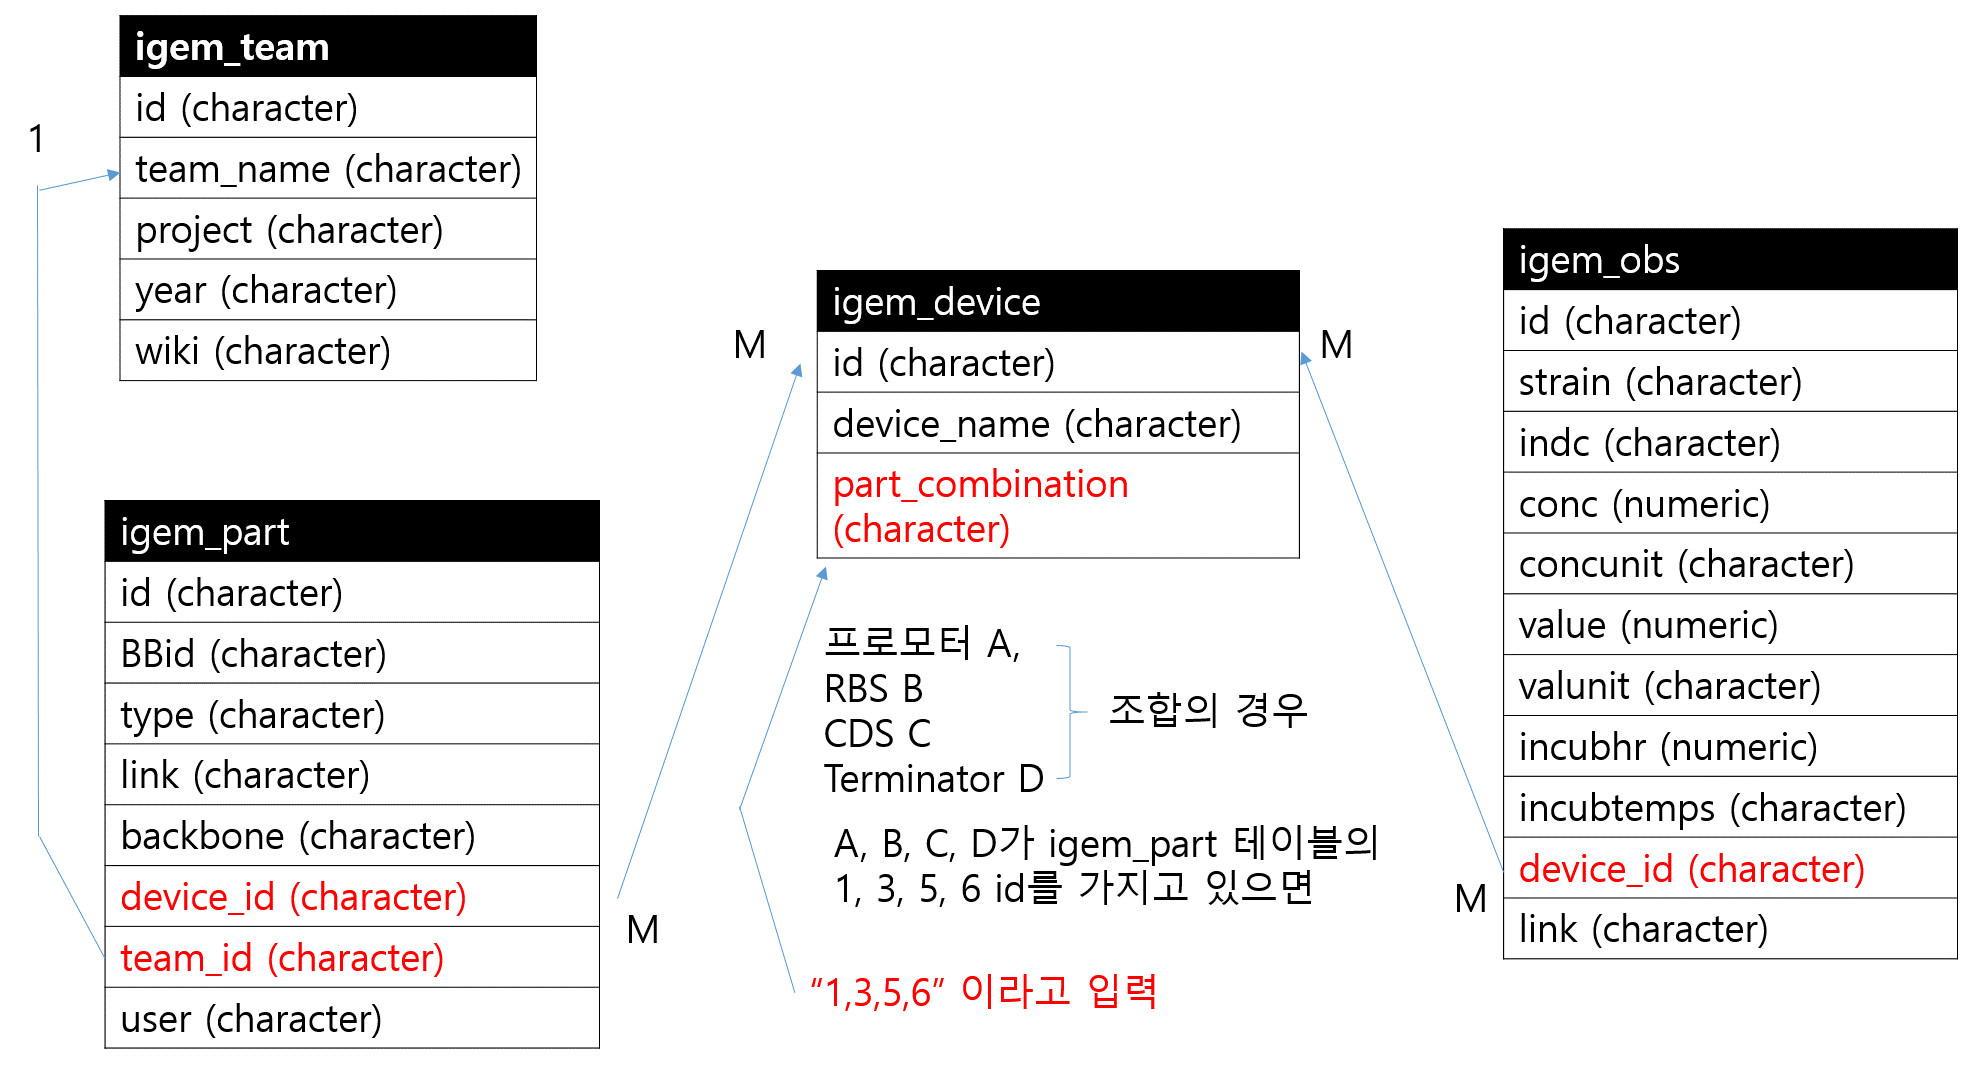
\includegraphics{_site/다운로드 (1).png}
  \caption{Data processing}
  \end{figure}
\item
  최종 데이터를 모두 합하면 동일한 ID를 갖는 데이터가 발생할 수 있음. 이
  경우 최종 데이터 병합 후 테이블 간의 연관성이 유지되지 않음. 따라서
  병합 전에 각 엑셀파일 이름에 사용자 id를 추가하여 데이터를 병합함.
\item
  각 엑셀파일에 사용자 id를 추가하기 위해 tmp \%\textgreater\%
  mutate(filename=filenames{[}i{]}) 함수를 이용해 사용자 id를 추가함.
\end{itemize}

\begin{Shaded}
\begin{Highlighting}[]
\FunctionTok{library}\NormalTok{(tidyverse)}
\end{Highlighting}
\end{Shaded}

\begin{verbatim}
## -- Attaching packages --------------------------------------- tidyverse 1.3.0 --
\end{verbatim}

\begin{verbatim}
## v ggplot2 3.3.4     v purrr   0.3.4
## v tibble  3.1.0     v dplyr   1.0.5
## v tidyr   1.1.3     v stringr 1.4.0
## v readr   1.4.0     v forcats 0.5.1
\end{verbatim}

\begin{verbatim}
## Warning: package 'ggplot2' was built under R version 4.0.5
\end{verbatim}

\begin{verbatim}
## -- Conflicts ------------------------------------------ tidyverse_conflicts() --
## x dplyr::filter() masks stats::filter()
## x dplyr::lag()    masks stats::lag()
\end{verbatim}

\begin{Shaded}
\begin{Highlighting}[]
\FunctionTok{library}\NormalTok{(magrittr)}
\end{Highlighting}
\end{Shaded}

\begin{verbatim}
## 
## Attaching package: 'magrittr'
\end{verbatim}

\begin{verbatim}
## The following object is masked from 'package:purrr':
## 
##     set_names
\end{verbatim}

\begin{verbatim}
## The following object is masked from 'package:tidyr':
## 
##     extract
\end{verbatim}

\begin{Shaded}
\begin{Highlighting}[]
\DocumentationTok{\#\# 다운로드 받은 엑셀 파일들 }
\NormalTok{filenames }\OtherTok{\textless{}{-}} \FunctionTok{dir}\NormalTok{(}\AttributeTok{path =}\NormalTok{ destdir, }\AttributeTok{pattern =} \StringTok{"*\_partdb.xlsx"}\NormalTok{)}


\NormalTok{tmp1 }\OtherTok{\textless{}{-}} \FunctionTok{list}\NormalTok{()}
\NormalTok{tmp2 }\OtherTok{\textless{}{-}} \FunctionTok{list}\NormalTok{()}
\NormalTok{tmp3 }\OtherTok{\textless{}{-}} \FunctionTok{list}\NormalTok{()}
\NormalTok{tmp4 }\OtherTok{\textless{}{-}} \FunctionTok{list}\NormalTok{()}

\ControlFlowTok{for}\NormalTok{(i }\ControlFlowTok{in} \DecValTok{1}\SpecialCharTok{:}\FunctionTok{length}\NormalTok{(filenames)) \{}
\NormalTok{  destfile }\OtherTok{\textless{}{-}} \FunctionTok{paste0}\NormalTok{(destdir, filenames[i])}
  
\NormalTok{  tmp }\OtherTok{\textless{}{-}} \FunctionTok{read\_excel}\NormalTok{(destfile, }\AttributeTok{sheet =} \DecValTok{1}\NormalTok{, }\AttributeTok{skip =} \DecValTok{0}\NormalTok{, }\AttributeTok{col\_names =}\NormalTok{ T)}
\NormalTok{  tmp }\SpecialCharTok{\%\textless{}\textgreater{}\%} \FunctionTok{mutate}\NormalTok{(}\FunctionTok{across}\NormalTok{(}\SpecialCharTok{!}\FunctionTok{where}\NormalTok{(is.character), as.character)) }
\NormalTok{  tmp1[[i]] }\OtherTok{\textless{}{-}}\NormalTok{ tmp }\SpecialCharTok{\%\textgreater{}\%} \FunctionTok{mutate}\NormalTok{(}\AttributeTok{filename=}\NormalTok{filenames[i])}
  
\NormalTok{  tmp }\OtherTok{\textless{}{-}} \FunctionTok{read\_excel}\NormalTok{(destfile, }\AttributeTok{sheet =} \DecValTok{2}\NormalTok{, }\AttributeTok{skip =} \DecValTok{0}\NormalTok{, }\AttributeTok{col\_names =}\NormalTok{ T)}
\NormalTok{  tmp }\SpecialCharTok{\%\textless{}\textgreater{}\%} \FunctionTok{mutate}\NormalTok{(}\FunctionTok{across}\NormalTok{(}\SpecialCharTok{!}\FunctionTok{where}\NormalTok{(is.character), as.character)) }
\NormalTok{  tmp2[[i]] }\OtherTok{\textless{}{-}}\NormalTok{ tmp }\SpecialCharTok{\%\textgreater{}\%} \FunctionTok{mutate}\NormalTok{(}\AttributeTok{filename=}\NormalTok{filenames[i])}
  
\NormalTok{  tmp }\OtherTok{\textless{}{-}} \FunctionTok{read\_excel}\NormalTok{(destfile, }\AttributeTok{sheet =} \DecValTok{3}\NormalTok{, }\AttributeTok{skip =} \DecValTok{0}\NormalTok{, }\AttributeTok{col\_names =}\NormalTok{ T)}
\NormalTok{  tmp }\SpecialCharTok{\%\textless{}\textgreater{}\%} \FunctionTok{mutate}\NormalTok{(}\FunctionTok{across}\NormalTok{(}\SpecialCharTok{!}\FunctionTok{where}\NormalTok{(is.character), as.character)) }
\NormalTok{  tmp3[[i]] }\OtherTok{\textless{}{-}}\NormalTok{ tmp }\SpecialCharTok{\%\textgreater{}\%} \FunctionTok{mutate}\NormalTok{(}\AttributeTok{filename=}\NormalTok{filenames[i])}
  
\NormalTok{  tmp }\OtherTok{\textless{}{-}} \FunctionTok{read\_excel}\NormalTok{(destfile, }\AttributeTok{sheet =} \DecValTok{4}\NormalTok{, }\AttributeTok{skip =} \DecValTok{0}\NormalTok{, }\AttributeTok{col\_names =}\NormalTok{ T) }
\NormalTok{  tmp }\SpecialCharTok{\%\textless{}\textgreater{}\%} \FunctionTok{mutate}\NormalTok{(}\FunctionTok{across}\NormalTok{(}\SpecialCharTok{!}\FunctionTok{where}\NormalTok{(is.character), as.character)) }
\NormalTok{  tmp4[[i]] }\OtherTok{\textless{}{-}}\NormalTok{ tmp }\SpecialCharTok{\%\textgreater{}\%} \FunctionTok{mutate}\NormalTok{(}\AttributeTok{filename=}\NormalTok{filenames[i])}
  
\NormalTok{\}}

\NormalTok{igem\_team }\OtherTok{\textless{}{-}} \FunctionTok{do.call}\NormalTok{(bind\_rows, tmp1)}
\NormalTok{igem\_part }\OtherTok{\textless{}{-}} \FunctionTok{do.call}\NormalTok{(bind\_rows, tmp2)}
\NormalTok{igem\_device }\OtherTok{\textless{}{-}} \FunctionTok{do.call}\NormalTok{(bind\_rows, tmp3)}
\NormalTok{igem\_obs }\OtherTok{\textless{}{-}} \FunctionTok{do.call}\NormalTok{(bind\_rows, tmp4)}
\end{Highlighting}
\end{Shaded}

\hypertarget{uxd14cuxc774uxbe14-uxac04-uxb370uxc774uxd130-uxc5f0uxacb0-uxbc0f-uxd1b5uxd569}{%
\subsubsection{테이블 간 데이터 연결 및
통합}\label{uxd14cuxc774uxbe14-uxac04-uxb370uxc774uxd130-uxc5f0uxacb0-uxbc0f-uxd1b5uxd569}}

\begin{itemize}
\tightlist
\item
  igem\_part와 igem\_team 데이터 테이블의 경우 team\_id와 filename을
  이용해 통합함.
\end{itemize}

\begin{Shaded}
\begin{Highlighting}[]
\FunctionTok{library}\NormalTok{(tidyverse)}

\DocumentationTok{\#\# new id }
\NormalTok{tmpdat }\OtherTok{\textless{}{-}}\NormalTok{ igem\_part }\SpecialCharTok{\%\textgreater{}\%} 
  \FunctionTok{left\_join}\NormalTok{(igem\_team, }\AttributeTok{by=}\FunctionTok{c}\NormalTok{(}\StringTok{"team\_id"}\OtherTok{=}\StringTok{"id"}\NormalTok{, }\StringTok{"filename"}\OtherTok{=}\StringTok{"filename"}\NormalTok{))}

\NormalTok{tmpdat }\OtherTok{\textless{}{-}}\NormalTok{ igem\_part }\SpecialCharTok{\%\textgreater{}\%} 
  \FunctionTok{full\_join}\NormalTok{(igem\_team, }\AttributeTok{by=}\FunctionTok{c}\NormalTok{(}\StringTok{"team\_id"}\OtherTok{=}\StringTok{"id"}\NormalTok{, }\StringTok{"filename"}\OtherTok{=}\StringTok{"filename"}\NormalTok{)) }\SpecialCharTok{\%\textgreater{}\%} 
  \FunctionTok{select}\NormalTok{(id, BBid, type, backbone, device\_id, user, filename, team\_name, year) }\SpecialCharTok{\%\textgreater{}\%} 
  \FunctionTok{drop\_na}\NormalTok{()}

\NormalTok{tmpdat2 }\OtherTok{\textless{}{-}}\NormalTok{ igem\_obs }\SpecialCharTok{\%\textgreater{}\%}
  \FunctionTok{full\_join}\NormalTok{(igem\_device, }\AttributeTok{by=}\FunctionTok{c}\NormalTok{(}\StringTok{"device\_id"}\OtherTok{=}\StringTok{"id"}\NormalTok{, }\StringTok{"filename"}\OtherTok{=}\StringTok{"filename"}\NormalTok{)) }\SpecialCharTok{\%\textgreater{}\%}
  \FunctionTok{select}\NormalTok{(id,strain,indc,conc,concunit,value,valunit,incubhr,incubtemp,device\_id,device\_name,part\_combination,filename) }\SpecialCharTok{\%\textgreater{}\%}
  \FunctionTok{drop\_na}\NormalTok{()}
\end{Highlighting}
\end{Shaded}

\begin{itemize}
\item
  select(column name1, column name2, \ldots) 함수를 통해 필요한 변수만
  선택하는 코드를 추가할 수 있음.
\item
  drop\_na()를 통해 선택한 변수의 데이터 중 NA가 있는 row를 제거할 수
  있음.
\item
  igem\_obs와 igem\_device는 device\_id와 filename을 이용해 통합함.
\item
  통합한 데이터를 가지고 실험 결과를 그래프로 나타낼 수 있음.
\end{itemize}

\begin{Shaded}
\begin{Highlighting}[]
\NormalTok{tmpdat }\SpecialCharTok{\%\textgreater{}\%} 
  \FunctionTok{filter}\NormalTok{(BBid}\SpecialCharTok{==}\StringTok{"BBa\_I0500"}\NormalTok{)}
\end{Highlighting}
\end{Shaded}

\begin{verbatim}
## # A tibble: 2 x 9
##   id    BBid    type    backbone device_id user    filename      team_name year 
##   <chr> <chr>   <chr>   <chr>    <chr>     <chr>   <chr>         <chr>     <chr>
## 1 1     BBa_I0~ Promot~ NA       1         gpemel~ gpemelianov_~ Jilin_Ch~ 2020 
## 2 5     BBa_I0~ Promot~ pSC101   2         gpemel~ gpemelianov_~ BHSF_ND   2019
\end{verbatim}

\begin{Shaded}
\begin{Highlighting}[]
\NormalTok{tmpd }\OtherTok{\textless{}{-}}\NormalTok{tmpdat2 }\SpecialCharTok{\%\textgreater{}\%} 
  \FunctionTok{mutate}\NormalTok{(}\AttributeTok{partcomb =} \FunctionTok{lapply}\NormalTok{(}\FunctionTok{strsplit}\NormalTok{(tmpdat2}\SpecialCharTok{$}\NormalTok{part\_combination, }\AttributeTok{split=}\StringTok{","}\NormalTok{), as.numeric)) }\SpecialCharTok{\%\textgreater{}\%} 
  \FunctionTok{filter}\NormalTok{(}\FunctionTok{unlist}\NormalTok{(}\FunctionTok{lapply}\NormalTok{(partcomb, }\ControlFlowTok{function}\NormalTok{(x)\{}\DecValTok{1} \SpecialCharTok{\%in\%}\NormalTok{ x\})) }\SpecialCharTok{\&}\NormalTok{ filename}\SpecialCharTok{==}\StringTok{"gpemelianov\_partdb.xlsx"}\NormalTok{)}

\NormalTok{finaldat }\OtherTok{\textless{}{-}}\NormalTok{ tmpd}

\NormalTok{tmpd }\OtherTok{\textless{}{-}}\NormalTok{tmpdat2 }\SpecialCharTok{\%\textgreater{}\%} 
  \FunctionTok{mutate}\NormalTok{(}\AttributeTok{partcomb =} \FunctionTok{lapply}\NormalTok{(}\FunctionTok{strsplit}\NormalTok{(tmpdat2}\SpecialCharTok{$}\NormalTok{part\_combination, }\AttributeTok{split=}\StringTok{","}\NormalTok{), as.numeric)) }\SpecialCharTok{\%\textgreater{}\%} 
  \FunctionTok{filter}\NormalTok{(}\FunctionTok{unlist}\NormalTok{(}\FunctionTok{lapply}\NormalTok{(partcomb, }\ControlFlowTok{function}\NormalTok{(x)\{}\DecValTok{5} \SpecialCharTok{\%in\%}\NormalTok{ x\})) }\SpecialCharTok{\&}\NormalTok{ filename}\SpecialCharTok{==}\StringTok{"gpemelianov\_partdb.xlsx"}\NormalTok{)}

\NormalTok{finaldat }\OtherTok{\textless{}{-}} \FunctionTok{bind\_rows}\NormalTok{(finaldat, tmpd)}

\NormalTok{plotdat }\OtherTok{\textless{}{-}}\NormalTok{ finaldat }\SpecialCharTok{\%\textgreater{}\%} 
  \FunctionTok{select}\NormalTok{(}\SpecialCharTok{{-}}\FunctionTok{c}\NormalTok{(id, filename, part\_combination, partcomb)) }\SpecialCharTok{\%\textgreater{}\%} 
  \FunctionTok{mutate}\NormalTok{(}\AttributeTok{value =} \FunctionTok{as.numeric}\NormalTok{(value))}

\NormalTok{plotdat }\SpecialCharTok{\%\textgreater{}\%}\NormalTok{ str}
\end{Highlighting}
\end{Shaded}

\begin{verbatim}
## tibble[,10] [10 x 10] (S3: tbl_df/tbl/data.frame)
##  $ strain     : chr [1:10] "E.coli" "E.coli" "E.coli" "E.coli" ...
##  $ indc       : chr [1:10] "Arabinose" "Arabinose" "Arabinose" "Arabinose" ...
##  $ conc       : chr [1:10] "0.02" "0.2" "2" "0" ...
##  $ concunit   : chr [1:10] "mM" "mM" "mM" "mM" ...
##  $ value      : num [1:10] 3000 8200 8000 250 500 600 750 2000 5000 10000
##  $ valunit    : chr [1:10] "Fluorescence" "Fluorescence" "Fluorescence" "a.u." ...
##  $ incubhr    : chr [1:10] "12" "12" "12" "4" ...
##  $ incubtemp  : chr [1:10] "NA" "NA" "NA" "37" ...
##  $ device_id  : chr [1:10] "1" "1" "1" "2" ...
##  $ device_name: chr [1:10] "D0001" "D0001" "D0001" "D0002" ...
\end{verbatim}

\begin{Shaded}
\begin{Highlighting}[]
\NormalTok{datasummary }\OtherTok{\textless{}{-}}\NormalTok{ plotdat }\SpecialCharTok{\%\textgreater{}\%} 
  \FunctionTok{group\_by}\NormalTok{(indc, conc) }\SpecialCharTok{\%\textgreater{}\%} 
  \FunctionTok{summarise}\NormalTok{(}\AttributeTok{mean=}\FunctionTok{mean}\NormalTok{(value), }\AttributeTok{n=}\FunctionTok{n}\NormalTok{()) }
\end{Highlighting}
\end{Shaded}

\begin{verbatim}
## `summarise()` has grouped output by 'indc'. You can override using the `.groups` argument.
\end{verbatim}

\begin{Shaded}
\begin{Highlighting}[]
\FunctionTok{ggplot}\NormalTok{(datasummary, }\FunctionTok{aes}\NormalTok{(}\AttributeTok{x=}\NormalTok{conc, }\AttributeTok{y=}\NormalTok{mean)) }\SpecialCharTok{+}
  \FunctionTok{geom\_bar}\NormalTok{(}\AttributeTok{stat=}\StringTok{"identity"}\NormalTok{) }\SpecialCharTok{+}
  \FunctionTok{theme\_bw}\NormalTok{()}
\end{Highlighting}
\end{Shaded}

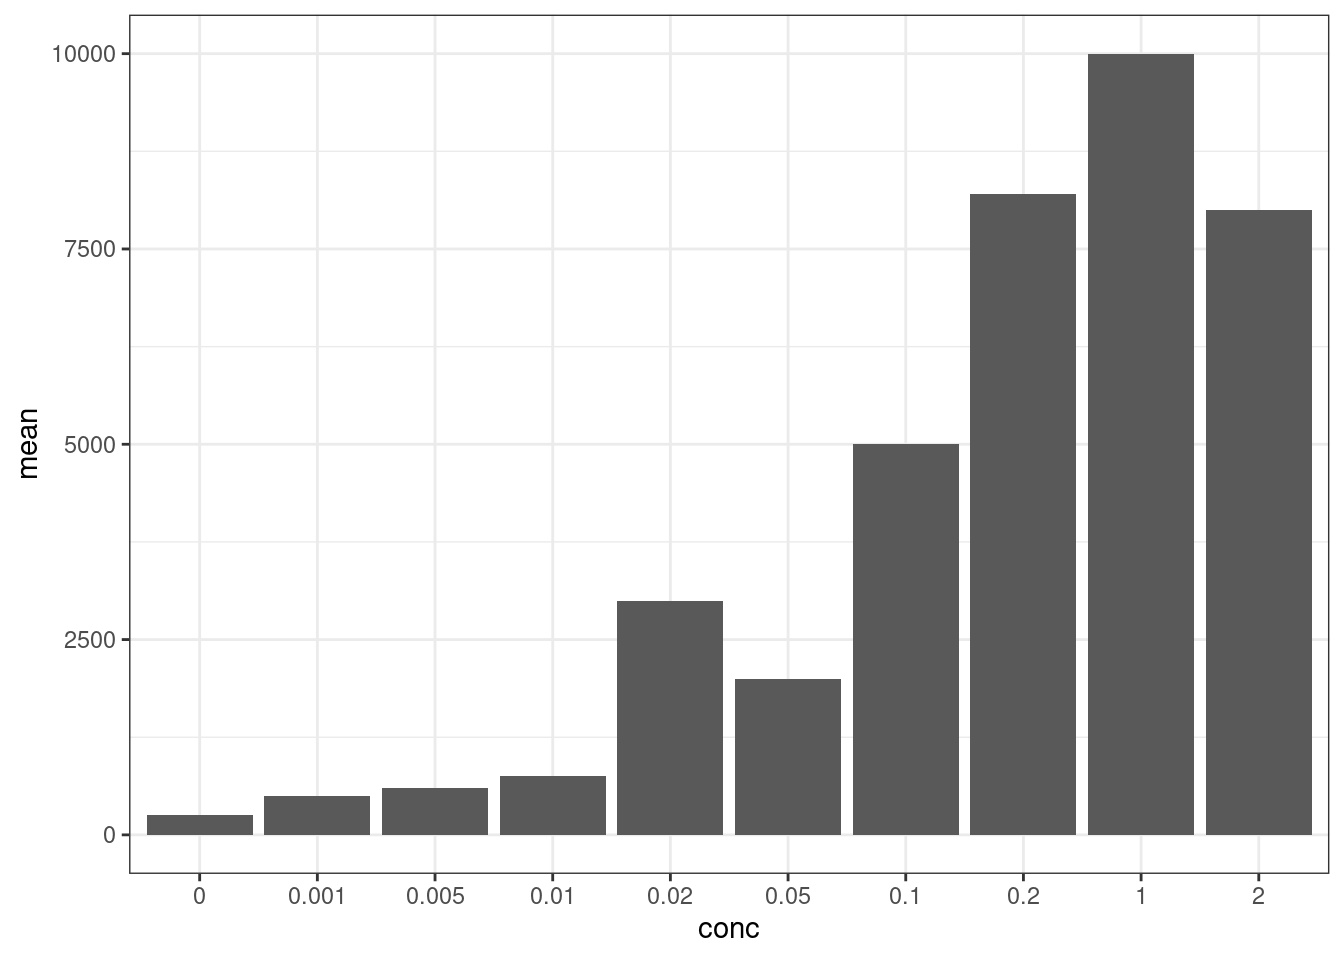
\includegraphics{Field-research-report_files/figure-latex/unnamed-chunk-8-1.pdf}

\begin{Shaded}
\begin{Highlighting}[]
\FunctionTok{library}\NormalTok{(tidyverse)}

\NormalTok{tmpdat }\SpecialCharTok{\%\textgreater{}\%} 
  \FunctionTok{filter}\NormalTok{(BBid}\SpecialCharTok{==}\StringTok{"BBa\_R0062"}\NormalTok{)}
\end{Highlighting}
\end{Shaded}

\begin{verbatim}
## # A tibble: 3 x 9
##   id    BBid    type    backbone device_id user    filename      team_name year 
##   <chr> <chr>   <chr>   <chr>    <chr>     <chr>   <chr>         <chr>     <chr>
## 1 5     BBa_R0~ promot~ PSB3K3   1         JinjuL~ jinjulee119_~ iBowu-Ch~ 2019 
## 2 8     BBa_R0~ Regula~ pACYC184 2         JinjuL~ jinjulee119_~ OUC-China 2020 
## 3 10    BBa_R0~ Promot~ -        3         sb.h    treebird19_p~ Stockholm 2020
\end{verbatim}

\begin{Shaded}
\begin{Highlighting}[]
\NormalTok{tmpd }\OtherTok{\textless{}{-}}\NormalTok{tmpdat2 }\SpecialCharTok{\%\textgreater{}\%} 
  \FunctionTok{mutate}\NormalTok{(}\AttributeTok{partcomb =} \FunctionTok{lapply}\NormalTok{(}\FunctionTok{strsplit}\NormalTok{(tmpdat2}\SpecialCharTok{$}\NormalTok{part\_combination, }\AttributeTok{split=}\StringTok{","}\NormalTok{), as.numeric)) }\SpecialCharTok{\%\textgreater{}\%} 
  \FunctionTok{filter}\NormalTok{(}\FunctionTok{unlist}\NormalTok{(}\FunctionTok{lapply}\NormalTok{(partcomb, }\ControlFlowTok{function}\NormalTok{(x)\{}\DecValTok{1} \SpecialCharTok{\%in\%}\NormalTok{ x\})) }\SpecialCharTok{\&}\NormalTok{ filename}\SpecialCharTok{==}\StringTok{"jinjulee119\_partdb.xlsx"}\NormalTok{)}

\NormalTok{finaldat }\OtherTok{\textless{}{-}}\NormalTok{ tmpd}

\NormalTok{tmpd }\OtherTok{\textless{}{-}}\NormalTok{tmpdat2 }\SpecialCharTok{\%\textgreater{}\%} 
  \FunctionTok{mutate}\NormalTok{(}\AttributeTok{partcomb =} \FunctionTok{lapply}\NormalTok{(}\FunctionTok{strsplit}\NormalTok{(tmpdat2}\SpecialCharTok{$}\NormalTok{part\_combination, }\AttributeTok{split=}\StringTok{","}\NormalTok{), as.numeric)) }\SpecialCharTok{\%\textgreater{}\%} 
  \FunctionTok{filter}\NormalTok{(}\FunctionTok{unlist}\NormalTok{(}\FunctionTok{lapply}\NormalTok{(partcomb, }\ControlFlowTok{function}\NormalTok{(x)\{}\DecValTok{5} \SpecialCharTok{\%in\%}\NormalTok{ x\})) }\SpecialCharTok{\&}\NormalTok{ filename}\SpecialCharTok{==}\StringTok{"jinjulee119\_partdb.xlsx"}\NormalTok{)}

\NormalTok{finaldat }\OtherTok{\textless{}{-}} \FunctionTok{bind\_rows}\NormalTok{(finaldat, tmpd)}

\NormalTok{plotdat }\OtherTok{\textless{}{-}}\NormalTok{ finaldat }\SpecialCharTok{\%\textgreater{}\%} 
  \FunctionTok{select}\NormalTok{(}\SpecialCharTok{{-}}\FunctionTok{c}\NormalTok{(id, filename, part\_combination, partcomb)) }\SpecialCharTok{\%\textgreater{}\%} 
  \FunctionTok{mutate}\NormalTok{(}\AttributeTok{value =} \FunctionTok{as.numeric}\NormalTok{(value))}

\NormalTok{plotdat }\SpecialCharTok{\%\textgreater{}\%}\NormalTok{ str}
\end{Highlighting}
\end{Shaded}

\begin{verbatim}
## tibble[,10] [12 x 10] (S3: tbl_df/tbl/data.frame)
##  $ strain     : chr [1:12] "cell-free" "cell-free" "cell-free" "cell-free" ...
##  $ indc       : chr [1:12] "AHL" "AHL" "AHL" "AHL" ...
##  $ conc       : chr [1:12] "0.1" "1" "10" "100" ...
##  $ concunit   : chr [1:12] "nM" "nM" "nM" "nM" ...
##  $ value      : num [1:12] 10 100 200000 300000 400000 350000 10 100 200000 300000 ...
##  $ valunit    : chr [1:12] "FLU" "FLU" "FLU" "FLU" ...
##  $ incubhr    : chr [1:12] "15" "15" "15" "15" ...
##  $ incubtemp  : chr [1:12] "37" "37" "37" "37" ...
##  $ device_id  : chr [1:12] "1" "1" "1" "1" ...
##  $ device_name: chr [1:12] "D0001" "D0001" "D0001" "D0001" ...
\end{verbatim}

\begin{Shaded}
\begin{Highlighting}[]
\NormalTok{datasummary }\OtherTok{\textless{}{-}}\NormalTok{ plotdat }\SpecialCharTok{\%\textgreater{}\%} 
  \FunctionTok{group\_by}\NormalTok{(indc, conc) }\SpecialCharTok{\%\textgreater{}\%} 
  \FunctionTok{summarise}\NormalTok{(}\AttributeTok{mean=}\FunctionTok{mean}\NormalTok{(value), }\AttributeTok{n=}\FunctionTok{n}\NormalTok{()) }
\end{Highlighting}
\end{Shaded}

\begin{verbatim}
## `summarise()` has grouped output by 'indc'. You can override using the `.groups` argument.
\end{verbatim}

\begin{Shaded}
\begin{Highlighting}[]
\FunctionTok{ggplot}\NormalTok{(datasummary, }\FunctionTok{aes}\NormalTok{(}\AttributeTok{x=}\NormalTok{conc, }\AttributeTok{y=}\NormalTok{mean, }\AttributeTok{fill=}\NormalTok{conc)) }\SpecialCharTok{+}
  \FunctionTok{geom\_bar}\NormalTok{(}\AttributeTok{stat=}\StringTok{"identity"}\NormalTok{) }\SpecialCharTok{+}
  \FunctionTok{theme\_bw}\NormalTok{()}\SpecialCharTok{+}
  \FunctionTok{scale\_fill\_brewer}\NormalTok{(}\AttributeTok{palette=}\StringTok{"Blues"}\NormalTok{)}
\end{Highlighting}
\end{Shaded}

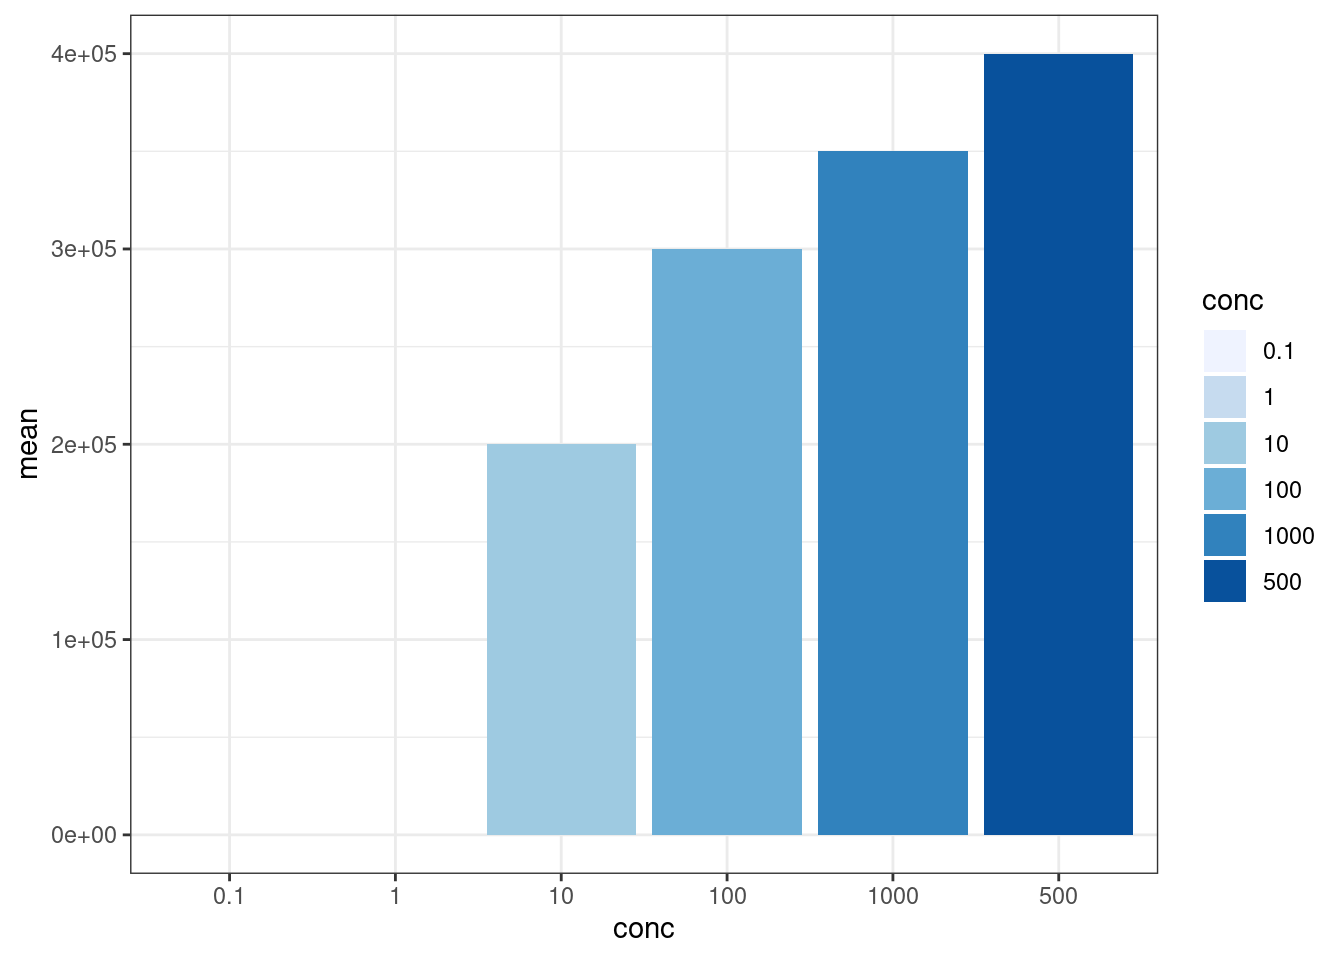
\includegraphics{Field-research-report_files/figure-latex/unnamed-chunk-9-1.pdf}

\begin{itemize}
\item
  위 결과는 여러 사람이 모은 데이터가 아니고, 반복 측정된 데이터가
  없어서 재현성을 확인할 수는 없음.
\item
  다른 part들에 대해서도 동일한 방법으로 분석을 수행할 수 있으며, 여러
  사람이 참여해서 데이터가 충분히 많아질 경우 하나의 부품이 얼마나 많은
  편차를 가지고 있는지에 대한 의미 있는 결과를 얻을 수도 있음.
\end{itemize}

\hypertarget{uxc5f0uxad6c-uxacb0uxacfc-4-uxd648uxd398uxc774uxc9c0-uxb9ccuxb4e4uxae30}{%
\subsection{연구 결과 4 : 홈페이지
만들기}\label{uxc5f0uxad6c-uxacb0uxacfc-4-uxd648uxd398uxc774uxc9c0-uxb9ccuxb4e4uxae30}}

link: \url{https://jinjulee119.github.io/researcheweb/}

\begin{itemize}
\item
  R markdown 파일을 html로 compile하여 웹사이트의 각 탭을 생성함.
\item
  ``My ResearchE Class Website''라는 이름의 홈페이지를 만들어 Home,
  About, Introduction 등 5개의 tab을 생성함.
\item
  홈페이지에 표시할 내용을 작성한 R markdown 파일을 만들고, knit로 html
  파일을 생성함.
\end{itemize}

name: ``My ResearchE Class Website''

navbar:

title: ``My ResearchE Class Website''

left:

\begin{verbatim}
- text: "Home"

  href: index.html

- text: "About"

  href: about.html
\end{verbatim}

\begin{itemize}
\item
  위 내용으로 text file을 작성, \_site.yml 파일로 저장함.
\item
  웹사이트의 각 탭에 필요한 내용을 작성할 수 있음.
\item
  예시 Introduction : 생물학의 반복성과 재현성 극복을 위한 소프트웨어
  (R, Rstudio, Rmarkdown, git) 활용, 협업 (data sharing), 합성생물학
  데이터 수집 등 Method \& Results : 배운 내용들 정리 (ex. Rstudio, git,
  rmarkdown 사용법, 합성생물학 데이터 수집 방법 등), submenu를 만들어서
  각 주제별로 Rmd 파일 만드는 것도 좋음 Discussion
\end{itemize}

\hypertarget{uxace0uxcc30}{%
\section{고찰}\label{uxace0uxcc30}}

\hypertarget{rstudiormarkdownuxc744-uxc774uxc6a9uxd55c-uxb370uxc774uxd130-uxcc98uxb9ac}{%
\subsection{Rstudio/Rmarkdown을 이용한 데이터
처리}\label{rstudiormarkdownuxc744-uxc774uxc6a9uxd55c-uxb370uxc774uxd130-uxcc98uxb9ac}}

\begin{itemize}
\item
  예시로 주어진 I0500 외에 다른 바이오부품에 대해서도 분석을 수행할 수
  있음.
\item
  직접 데이터를 수집한 R0062에 대해서도 동일한 방법으로 그래프를
  만들어봄. 그래프 작성 시 fill, scale\_fill\_brewer 등의 부가적인
  기능을 부여하여 그래프를 작성함.
\item
  이번 수업에서는 하나의 파트에 대해 한 사람이 조사한 결과에서만
  데이터를 분석했지만 여러 연구자가 수행한 동일한 실험 데이터를 분석할
  경우 Rstuio를 통해 해당 실험의 반복성을 확인하기 용이함.
\end{itemize}

\hypertarget{uxb370uxc774uxd130-uxd1b5uxd569-uxacfcuxc815uxc5d0uxc11cuxc758-uxc624uxb958-uxd574uxacb0}{%
\subsection{데이터 통합 과정에서의 오류
해결}\label{uxb370uxc774uxd130-uxd1b5uxd569-uxacfcuxc815uxc5d0uxc11cuxc758-uxc624uxb958-uxd574uxacb0}}

tmpdat2 \textless- igem\_obs \%\textgreater\%

full\_join(igem\_device, by=c(``device\_id''=``id'',
``filename''=``filename'')) \%\textgreater\%

drop\_na()

tmpdat2 \%\textgreater\% str

\begin{itemize}
\item
  위 코드를 수행할 경우 tmpmdat2 table에 변수만 15개고, 데이터가 모두
  사라짐.
\item
  0 obs. of 15 variables, 15개의 column을 가지고 있지만 data가 없는
  table로 만들어짐.
\item
  이유를 파악해본 결과, igem\_obs와 igem\_device 데이터 테이블에 NA가
  매우 많음. 사용자에 따라 igem\_obs의 promoter column이 없는 경우도
  있고, strain 데이터가 없는 경우도 발견됨.
\item
  결과적으로 drop\_na() 코드로 인해 NA가 포함된 모든 row가 제거됨.
\item
  따라서 이를 수정하기 위해 NA가 없는 column을 지정해주면 해당
  column에서 NA가 있는 row만 제거해야 함.
\end{itemize}

tmpdat2 \textless- igem\_obs \%\textgreater\%

full\_join(igem\_device, by=c(``device\_id''=``id'',
``filename''=``filename''))

\begin{itemize}
\tightlist
\item
  위 코드를 수행할 경우 table of 146 obs. of 15 variables
\end{itemize}

tmpdat2 \textless- igem\_obs \%\textgreater\%

full\_join(igem\_device, by=c(``device\_id''=``id'',
``filename''=``filename'')) \%\textgreater\%

select(id,strain,indc,conc,concunit,value,valunit,incubhr,incubtemp,device\_id,device\_name,part\_combination,filename)
\%\textgreater\%

drop\_na()

\begin{itemize}
\tightlist
\item
  위 코드를 수행하여 NA가 다량 포함된 column을 제외하고 로딩할 경우
  table of 115 obs. of 13 variables가 정상적으로 생성됨.
\end{itemize}

\end{document}
